\documentclass{article}

\usepackage[utf8]{inputenc}
\usepackage{amsfonts}
\usepackage{amsmath}
\usepackage{graphicx}
\usepackage{indentfirst}
\usepackage{polski}

\begin{document}

\section{Dystanse}

Aby znajdować grupy wyborców, którzy głosują podobnie, trzeba na początku
zdefiniować, co to znaczy, że dwóch wyborców głosuje podobnie. W naszym modelu
głosem jest podzbiór projektów $A \subseteq C$. Chcemy zatem zdefiniować
funkcję podobieństwa głosów:
\[ s : 2^C \times 2^C \to \mathbb{R} \]

Czasami zamiast funkcji podobieństwa, łatwiej będzie mówić o funkcji
odległości. Jest to intuicyjnie równoważne: wyborcy są blisko siebie wtedy i
tylko wtedy gdy są podobni.

\subsection{Różne propozycje miar}

\subsubsection{Odległość Hamminga}

Jedną z intuicyjnych miar odległości, o których możemy pomyśleć, jest liczba
projektów, na których dwóch wyborców się różni -- czyli takich na które głosuje
dokładnie jeden z nich. Możemy zdefiniować ją wzorem:
\[ d_H(A,B) = |A \Delta B| \]

W podobny sposób możemy zdefiniować miarę podobieństwa jako liczbę projektów
na które głosują obaj wyborcy:
\[ s(A,B) = |A \cap B| = |A \cup B| - d_H(A,B) \]

\subsubsection*{Brak normalizacji}

Rozważmy następujących wyborców:
\begin{align*}
  A_{v_1} &= \{ a, c_1 \} \\
  A_{v_2} &= \{ b, c_1 \} \\
  A_{v_3} &= \{ a, c_1, c_2, c_3, c_4, c_5, c_6, c_7, c_8 \} \\
  A_{v_4} &= \{ b, c_1, c_2, c_3, c_4, c_5, c_6, c_7, c_8 \}
\end{align*}

Która para z nich głosuje podobniej: $v_1$ i $v_2$ czy $v_3$ i $v_4$?

Intuicyjnie powiedzielibyśmy, że druga. Można to tłumaczyć faktem, że spośród
10 projektów na które głosują $v_3$ i $v_4$, na aż 8 z nich się ze sobą
zgadzają. W przypdaku pierwszej pary jest to tylko jeden z trzech.

Natomiast gdy spojrzymy na odległości Hamminga, okażą się one równe:
\[ H(A_{v_1},A_{v_2}) = |\{a,b\}| = H(A_{v_3},A_{v_4}) \]

Analogiczny przypadek możemy skonstruować dla miary podobieństwa która liczy
przecięcie zbiorów.

\subsubsection{Odległość Jaccarda}

Powyższy przykład pokazuje, że powinniśmy odnieść liczbę projektów na których
wyborcy się nie zgadzają do ilości projektów na które głosują:
\[ d_J(A,B) = \frac{|A \Delta B|}{|A \cup B|} \]

Przy okazji otrzymaliśmy przydatną własność:
\[ d_J(A,B) \in [0, 1] \]

W związku z czym łatwo zdefiniować współczynnik (podobieństwa) Jaccarda:
\[ s_J(A,B) = 1 - d_J(A,B) = \frac{|A \cap B|}{|A \cup B|}, \]
znany również jako współczynnik IoU (Intersection over Union).

\subsubsection*{Pierwsze aksjomaty}

Aby usystematyzować rozpatrywane miary, zdefiniujmy kilka aksjomatów:

\begin{itemize}
  \item Normalizacja: $s(A,B),d(A,B) \in [0, 1]$
  \item Zwrotność: $s(A,A) = 1, d(A,A) = 0$
  \item Symetria: $s(A,B) = s(B,A), d(A,B) = d(B,A)$
  \item Nietówność trójkąta: $d(A,B) + d(B,C) \geq d(A,C)$
\end{itemize}

Jeżeli jakaś miara miara podobieństwa (odległości) spełnia własność
normalizacji, to możemy łatwo zdefiniować odpowiadającą jej miarę odległości
(podobieństwa):
\[ d(A,B) = 1 - s(A,B) \]

Spośród rozpatrywanych dotychczas miar, odległość Hamminga spełniała
symetrię, natomiast ze względu na to że nie była znormalizowana, to nie
spełniała też zwrotności. Odległość Jaccarda wszystkie cztery aksjomaty.

\subsubsection{SimRank}

Rozważmy następujące projekty i wyborców:
\begin{align*}
  c_1 &= \text{Sadzenie drzew przy ulicy Adama Mickiewicza} && A_{v_1} = \{c_1\} \\
  c_2 &= \text{Sadzenie drzew przy ulicy Juliusza Słowackiego} && A_{v_2} = \{c_2\} \\
  c_3 &= \text{Budowa elektorni węglowej} && A_{v_3} = \{c_3\}
\end{align*}

Intuicyjnie powiedzielibyśmy, że wborcy $v_1$ i $v_2$ są do siebie bardziej
podobni niż do wyborcy $v_3$. Wynika to z faktu, że projekty $c_1$ i $c_2$
są do siebie bardziej podobne niż do projektu $c_3$.

Motywuje to następującą intuicję: wyborcy są podobni, jeżeli głosują na podobne
projekty. Pozostaje nam zatem powiedzieć kiedy projekty są do siebie podobne.
Możemy to zrobić w dokładnie ten sam sposób: jeżeli głosują na nie podobni
wyborcy.

Powyższą intuicję możemy skonkretyzować, mówiąc że podobieństwo wyborców
(projektów) jest średnim podobieństwem projektów na które głosują (wyborców
którzy na nie głosują).

Mamy zatem dwie funkcje -- podobieństwa wyborców i projektów:
\begin{align*}
  s^V_R : V \times V \to [0, 1] \\
  s^C_R : C \times C \to [0, 1]
\end{align*}
Definiujemy $s^V_R(v,v)=s^C_R(c,c)=1$. Natomiast dla $v \neq u$ i $c \neq d$
mamy następujące równanie rekurencyjne:
\begin{align*}
  s^V_R(v, u) &= \frac{D}{|A_v| |A_u|} \sum_{c \in A_v} \sum_{d \in A_u} s^C_R(c, d) \\
  s^C_R(c, d) &= \frac{D}{|V_c| |V_d|} \sum_{v \in V_c} \sum_{u \in V_d} s^C_R(v, u)
\end{align*}
Gdzie $v_c$ to zbiór wyborców którzy głosują na proejkt $c$, a $D \in (0, 1)$
to współczynnik zanikania (decay), potrzebny do zbieżności metody iteracyjnej.

Tak zdefiniowana miara spełnia normalizację, zwrotność i symetrię. Warto
jednak zauważyć że zwrotność spełniamy w dość sztuczny sposób -- ustawiając
ją na sztywno w definicji. Natomiast dla różnych wyborców, maksymalne ich
podobieństwo wynosi $C$, co łatwo udowodnić korzystając ze zwrotności.

% TODO: czy nierówność trójkąta

\subsubsection{RoleSim}

\subsubsection*{Wyborcy jako wektory}

Przed przejściem do następnych miar, spójrzmy na wyborców jako wektory w
$d = |C|$ wymiarowej przestrzeni, w której każdy projekt ma swój wymiar. Wektor
wyborcy będzie miał 1 na danej współrzędnej, jeżeli głosuje na dany projekt,
a 0 w przeciwnym wypadku:
\[ \vec v = \sum_{i=1}^d \vec e_i [c_i \in A_v] \]

Zauważmy następującą intuicję: projekty na które głosuje dany wyborca
wyznaczają "kierunek w którym głosuje".

\subsubsection{Odległość Euklidesa}

Najbardziej oczywistą miarą, kiedy patrzymy na wyborców jak na wektory, jest
odległość euklidesa:
\[ d_E(\vec v, \vec u) = | \vec v - \vec u | \]

Spełnia ona symetrię oraz nierówność trójkąta, a jeżeli dodatkowo podzielimy
ją przez $\sqrt d$, to również normalizację i zwrotność.

\subsubsection{Podobieństwo cosinusów}

Trochę mniej oczywistą miarą, ale znacznie częściej używaną w praktyce, jest
podobieństwo cosinusów:
\[ d_C(\vec v, \vec u) = \frac{\vec v \cdot \vec u}{|\vec v||\vec u|} \]

Spełnia ona normalizację, zwrotność i symetrię, ale nie spełnia nierówności
trójkąta.

\subsubsection{Odległość cięciwowa (chord)}

Podążając za intuicją, że "wyborcy głosują w jakimś kierynku", możemy
znormalizować ich wektory. Wtedy liczba projektów na które głosują nie będzie
miała znaczenia, a liczyć się bedzie jedynie kierunek.
\[
  d_{Ch}(\vec v, \vec u) =
  \left|\frac{\vec v}{|\vec v|} - \frac{\vec u}{|\vec u|}\right|
\]

Zauważmy, że:
\begin{align*}
  d_{Ch}(\vec v, \vec u)^2
  &= \left|\frac{\vec v}{|\vec v|} - \frac{\vec u}{|\vec u|}\right|^2 \\
  &= \left|\frac{\vec v}{|\vec v|}\right|^2
   + \left|\frac{\vec u}{|\vec u|}\right|^2
   - 2 \left( \frac{\vec v}{|\vec v|} \cdot \frac{\vec u}{|\vec u|} \right) \\
  &= 2(1 - d_C(\vec v, \vec u))
\end{align*}

Czyli z dokładnością do przekształcenia afinicznego, ta odległość jest
pierwiastkiem z odległości cosinusów.

Jeżeli dodatkowo podzielimy tę odległość przez $\sqrt 2$, to będzie spełniać
normalizację, zwrotność, symetrię i nierówność trójkąta.

\subsubsection{Najkrótsza ścieżka w grafie dwudzielnym}

\subsection{Histogramy}

Aby lepiej zrozumieć rozważane miary podobieństwa, warto spojrzeć jak wygląda
ich rozkład wartości na konkretnych danych.

%\begin{figure}[h]
\noindent
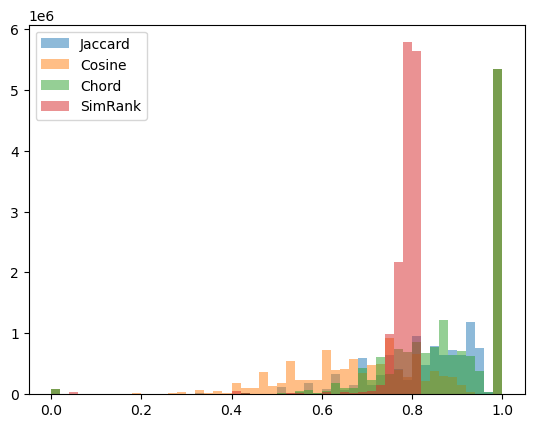
\includegraphics[width=\textwidth]{dist_hist.png}
%\end{figure}

\subsection{Korelacje}

Aby dowiedzieć się więcej o rozważanych miarach podobieństwa, możemy zbadać
korelacje między nimi.

\begin{center}
\begin{tabular}{|c|cccc|}
  \hline
    & Jaccard & Cosine & Chord & SimRank \\
  \hline
  Jaccard & 1.00 & 0.96 & 0.98 & 0.64 \\
  Cosine  & 0.96 & 1.00 & 0.97 & 0.57 \\
  Chord   & 0.98 & 0.97 & 1.00 & 0.71 \\
  SimRank & 0.64 & 0.58 & 0.71 & 1.00 \\
  \hline
\end{tabular}
\end{center}

\section{Wizualizacja}

Aby ocenić jakość wizualizacji, można zbadać korelację między odległością w
embeddingu a normalną.

\subsection{Metody}

\subsubsection{TSNE}

\subsubsection{MDS}

\subsubsection{PCA}

\subsubsection{UMAP?}

\subsubsection{LDA?}

\section{Community Detection}

\section{Klastrowanie}

\section{Ocena jakości klastrów}

\subsection{Różne współczynniki}

\subsubsection{Silhouette}

Dla każdego punktu ocenia jak dobrze został przydzielony do swojego klastra
liczbą z przedziału $[0,1]$.

\paragraph{Silhouette coefficient}

\[ SC = \max_k \tilde{s}(k) \]

Maksymalny średnia wartość Silhouette. Używana czasami do określenia jak
dobrze dana metoda klastrowania odnajduje klastry.

\subsubsection{Davies-Bouldin index}

\subsubsection{Dunn index}

\subsubsection{Calinski-Harabasz index}

\subsection{Walidacja lingwistyczna}

\section{Identyfikacja grup}

Zamiast podziału na klastry można próbować identyfikować podobne grupy.

\end{document}
